\documentclass[10pt, conference]{IEEEtran}
\IEEEoverridecommandlockouts
% The preceding line is only needed to identify funding in the first footnote. If that is unneeded, please comment it out.
\usepackage{cite}
\usepackage{amsmath,amssymb,amsfonts}
%\usepackage{algorithmic}
\usepackage{amsmath}
\usepackage{algorithm}
\usepackage[noend]{algpseudocode}
\usepackage{comment}
\usepackage{graphicx}
\usepackage{textcomp}
% Bobo Added
\usepackage{listings}
\usepackage{color}
\usepackage[justification=centering]{caption}
\def\BibTeX{{\rm B\kern-.05em{\sc i\kern-.025em b}\kern-.08em
    T\kern-.1667em\lower.7ex\hbox{E}\kern-.125emX}}
\begin{document}



\makeatletter
\def\BState{\State\hskip-\ALG@thistlm}
\makeatother


\title{Eliminating Power Side-Channel Leaks during Register Allocation\\
%{\footnotesize \textsuperscript{*}Note: Sub-titles are not captured in Xplore and should not be used}
%\thanks{Identify applicable funding agency here. If none, delete this.}
}

\author{\IEEEauthorblockN{Jingbo Wang, Chao Wang}
\IEEEauthorblockA{\textit{Department of Computer Science} \\
\textit{University of Southern California}\\
Los Angeles, USA \\
jingbow@usc.edu, wang626@usc.edu}
}

\maketitle

\begin{comment}
\begin{abstract}
This document is a model and instructions for \LaTeX.
This and the IEEEtran.cls file define the components of your paper [title, text, heads, etc.]. *CRITICAL: Do Not Use Symbols, Special Characters, Footnotes, 
or Math in Paper Title or Abstract.
\end{abstract}
\end{comment}

\begin{IEEEkeywords}
Verification, Mitigation, Cryptography, LLVM Compiler,  SMT Solver
\end{IEEEkeywords}

\section{Technical Background}
Side channel attacks allow attacker to infer the security-critical information of a system by observing its external behaviours, which are possible due to the presence of an underlying vulnerability. For example, in the case of timing channel, attackers can infer the relevant information about security-sensitive data by observing the execution time it takes to perform specific branches or some operations. After the introduction of execution timing channel as the first practical side channel to recover the secret key of implementation of cryptographic algorithms, other side-channel analysis approaches have been introduced later\cite{moradi2014side}. For instance, power consumption, acoustic, optical emission and temperature are those which have been brought to the attention of research community. For instance, power side channel attacks are feasible because the program exhibits different power consumptions based on the properties involving \emph{key}. Countermeasures proposed to overcome Simple Power Analysis (SPA) and Differential Power Analysis (DPA), are dummy instruction insertions, data masking, table masking, balancing bit-flips and so on. All these methods are either unable to cover all encryption algorithms or burden the system with high area cost and energy consumption.\cite{ambrose2007rijid}

    Hence, the most effective defense against side-channel attack is to eradicate the underlying vulnerabilities by ensuring the resource usage won't differ with respect to \emph{key}. In this work, we pay most attention to the power side channel. Recent works have explored some countermeasures for avoiding the power side channel and develop side-channel-free programs by automatically analyzing the correlations between difference in power consumption and variation in security-sensitive data. This work\cite{eldib2014synthesis} proposes new synthesis method for generating countermeasures for cryptographic software code, which takes an unprotected program as input and returns a functionally equivalent but power channel leak free new program as output. This countermeasure is based on the Hamming Weight model and is guaranteed to be perfectly masked in all intermediate results which is independent of \emph{key}. However, this work assumes that all the intermediate register will be distributed into distinct registers and estimate the power consumption on the basis of this assumption. After register allocation, there are multiple intermediate variables sharing the same register and this approach is still possible to leak secret information as the leakage model is not precise enough. Another work\cite{ambrose2007rijid} injects random instructions at random places during the execution of an application which protects the system from both SPA and DPA. But this solution is coarse-grained, it just choose a region and set random operations on this region. In order to minimize performance overhead, \cite{saab2016side} inserts two dummy loads before and after a collection of sensitive data loads and around any loads of changing data, such as input data. However, it will incur performance overhead and this analysis leak will reappear, presumably based on the Hamming weight of the state before the mixing of the round key in AES.

For the sake of solving the above problems existing in state of the art methods, we propose a more accurate leakage model and apply it to check whether the given source program has potential leakages. In addition, we also design a mitigation approach for generating power channel leak-free program. This practical countermeasure can be introduced in software to increase resistance and meet multiple security requirements. 
\section{Problem Statement}
The practical result\cite{moradi2014side} of using static power analysis to mount a successful power side-channel attack illustrated that the registers' content and gates' output should be the main leakage resource in FPGA platform. We apply this conclusion and the classic model\cite{brier2004correlation} used for the power consumption of cryptographic devices in our work to build the leakage model. Followings are leakage analysis of a source program under different power models and register allocation scenarios. With respect to this example, we will propose a more accurate leakage model for power channel which can explore more underlying vulnerabilities. In this section, we present an example owning potential power side channel leakage under finer-grained leakage model, and illustrate how this data leakage problem can be solved by our approach in \emph{Section III (Solution Section)}. 
\subsection{Motivating Example}
%In this section, we present the example and explain its functionality (which variables are secret, and how they are stored in registers of a CPU).
Given the \emph{leak()} function in Figure~\ref{example1}. Here we assume each input and the output are all 1-bit data. Input \emph{key} is the secret data while input \emph{i1,i2} and \emph{i3} are plaintext. The output \emph{n3} is regarded as the ciphertext and \emph{n1,n2} are both intermediate variables involving with the key and the plaintext value. This simple  cryptographic program consists of the linear($\oplus$) and non-linear($\wedge$) calculations. In order to verify this program is leak-free, we need to make sure that values of all the intermediate variables are statistically independent of \emph{key}. For instance, given different \emph{key} values and same plaintext inputs, if \emph{n1} exhibits various power channel behaviours, then it shows that the program in Figure~\ref{example1} exists side channel leakage, as there are \emph{key}-induced different power consumptions. To verify if there are some \emph{key}-induced differences in power consumption, we compare and apply different power analysis models in subsequent sections.

%\listoffigures
\begin{figure}[hbt!]
\centering
\begin{minipage}{.95\linewidth}
\begin{lstlisting}[language={[ANSI]C},numbers=left,numberstyle=\tiny, basicstyle=\ttfamily\small, frame=none]
int leak(int i1, int i2, int key, int i3)
{
	int n1,n2,n3;
	n1 = i1 ^ i2;
	n2 = (n1 ^ 1) ^ key;
	n3 = n2 & i3;
	return n3;
}

\end{lstlisting}
\end{minipage}
\caption{Example1 source code}
\label{example1}
\end{figure}

\subsection{No Leak under Hamming Weight (HW) Model}
%We explain why there is no leakage under the HW model...
In Hamming Weight power leakage model, one can mathematically describe the power consumption according to the computed bits(number of 1s in the intermediate byte value), which means there is a correlation between the Hamming Weight of the intermediate variables and the power consumption traces. In the example Fig~\ref{example1}, if Hamming Weights of the intermediate variables are independent of the \emph{key} value, then it can make sure that this program is power side channel leakage free. 
\\
According to the Table \ref{table:truth}, the value of intermediate variables \emph{n1,n2} are not dependent on the \emph{key} value, which means that the number of 1-bit is constant when \emph{key} differs. Under Hamming Weight model, we assume that the power leakage of the device correlates to the intermediate variables involved in the sensitive operations. All the intermediate variables \emph{n1,n2} have immutable number of 1-bit with different \emph{key} values, hence the power consumption won't change either. This program will be regarded as power side channel free as the resource usage won't differ as the \emph{key} value varies.
\begin{table}[htb!]
\centering
\begin{tabular}{|l|l|l|l|l|l|l|l|l|}
\hline
key & i1 & i2 & i3 & n1 & n2 & n3 & n1$\oplus$n2 & n2$\oplus$n3 \\ \hline\hline
0   & 0  & 0  & 0  & 0  & 1  & 0  & 1                     & 1                     \\ \hline
0   & 0  & 0  & 1  & 0  & 1  & 1  & 1                     & 0                     \\ \hline
0   & 0  & 1  & 0  & 1  & 0  & 0  & 1                     & 0                     \\ \hline
0   & 0  & 1  & 1  & 1  & 0  & 0  & 1                     & 0                     \\ \hline
0   & 1  & 0  & 0  & 1  & 0  & 0  & 1                     & 0                     \\ \hline
0   & 1  & 0  & 1  & 1  & 0  & 0  & 1                     & 0                     \\ \hline
0   & 1  & 1  & 0  & 0  & 1  & 0  & 1                     & 1                     \\ \hline
0   & 1  & 1  & 1  & 0  & 1  & 1  & 1                     & 0                     \\ \hline\hline
1   & 0  & 0  & 0  & 0  & 0  & 0  & 0                     & 0                     \\ \hline
1   & 0  & 0  & 1  & 0  & 0  & 0  & 0                     & 0                     \\ \hline
1   & 0  & 1  & 0  & 1  & 1  & 0  & 0                     & 1                     \\ \hline
1   & 0  & 1  & 1  & 1  & 1  & 1  & 0                     & 0                     \\ \hline
1   & 1  & 0  & 0  & 1  & 1  & 0  & 0                     & 1                     \\ \hline
1   & 1  & 0  & 1  & 1  & 1  & 1  & 0                     & 0                     \\ \hline
1   & 1  & 1  & 0  & 0  & 0  & 0  & 0                     & 0                     \\ \hline
1   & 1  & 1  & 1  & 0  & 0  & 0  & 0                     & 0                     \\ \hline
\end{tabular}
\caption{Truth Table of Example1}
\label{table:truth}
\end{table}

\subsection{No Leak under Hamming Distance (HD) Model}
%We explain why there is no leakage under the HD model either ...
Under Hamming Distance(HD) model, the data leakage through the power side-channel depends on the number of bits switching from one state to the other. In this case, the leakage current consumed is related to the number of 1-0 transit or 0-1 transit. In Hamming Distance model, there is a reference state to decide which the bits are switched. We assume this reference state is a constant value, \emph{R}. It will always be the same if the same data manipulation occurs at the same time. In the HD leakage model, the number of flipping bits to go from R to D is described by $HD(D, R)$ = $HW(D \oplus R)$ (The variable value $D = \sum _{ j=0 }^{ m-1 }{ { d }_{ j }{ 2 }^{ j } }$ with the bit values $ { d }_{ j } = 0$ or 1, $H(D) = \sum _{ j=0 }^{ m-1 }{ { d }_{ j } }$. Here we assume one bit, then m = 1). Actually, the Hamming Weight model is a specific case for HD model which assumes that R = 0. The assumption also propose a linear correlation between the current consumption and the $HD(D, R)$.
\\
As we can see from this example, for intermediate variable \emph{n1}, assuming R is 1, hence the average value of $HD(n1, R)$ is 0.5 under both cases that  \emph{key} equals to 1 or 0. While R is 0, the \emph{HD} value is also same under different \emph{key} values, which means that the Hamming Distance between intermediate variable \emph{n1} and R is constant as \emph{key} varies. Hence, the constant HD values represent the constant power consumption under different  \emph{key} values. In sum, the source code in Figure~\ref{example1} is also power leakage free under Hamming Distance model.
 \subsection{Leak after Register Allocation}
%We explain why, after register allocation, there is leakage under the HD model...
As previous research shows, the dependency of the leakage current to the register's content is clear. In Section A and B, we all assume that all intermediate variables are allocated to distinct registers. If the register value or value transition inside register have no correlation with the \emph{key}, which means the power consumptions have no relation with \emph{key}, then it's side channel leakage free. However, in specific target platform such as X86-64, diverse intermediate variables may reuse the same register. Under HW model, all intermediate values have no correlation with \emph{key} in program of Figure~\ref{example1}. If the intermediate values are stored in same register, which means sum of 1-bit the register owns equals to the sum of 1-bit from all the intermediate variables. As the register value is independent of \emph{key} as the intermediate variables, sum of the register values are also irrelevant to \emph{key}. Hence, the power consumption won't depend on the \emph{key} either.
\\
Nevertheless, under HD model, there are some leakage issues after the register allocation. Figure~\ref{example2} is the assembly code from this example in X86-64 system. \emph{i1,n1,n1$\oplus$key, n2} are stored in the same register \%edi. Most critically, two consecutive states of \%edi register will stores the value of \emph{n1}, \emph{n1$\oplus$key} as line 11 shows in Figure~\ref{example2}. We assume ${\%edx}_{1}$ represents \emph{n1}, ${\%edx}_{2}$ represents \emph{n1$\oplus$key}. In HD model, HD(${\%edx}_{1}, {\%edx}_{2}$) = HW(${\%edx}_{1} \oplus {\%edx}_{2}$) = HD(\emph{key}). Hence the amount of the 0-1 or 1-0 transitions between two states of the register \%edx will depend on \emph{key}, which means the power consumption will also have relation with the \emph{key} value. Therefore, this program still have power side-channel leakage after the register allocation. Meanwhile, we can also see from Table \ref{table:truth}, the value of \emph{n1} $\oplus$ \emph{n2} representing the number of transition bits between two successive states of the register keeps 1 when \emph{key} equals to 0, vice versa. Hence, as the number of transition bits inside a register depending on \emph{key} have correlation with power consumption, the \emph{key} value will definitely relate with the power consumption, which results in the side channel leakage. In other platforms such as ARM or MIPS, there are some intermediate variables sharing the same register as well. Therefore, under the Hamming Distance power analysis model and the register allocation scenario, the power channel leakage problem generally exists in various platforms.
\begin{figure}[hbt!]
\centering
\begin{minipage}{.65\linewidth}
\begin{lstlisting}[language={[ANSI]C},numbers=left,numberstyle=\tiny, basicstyle=\ttfamily\small, frame=none]
leak:                                   # @leak
	.cfi_startproc
# BB#0:                                 # %entry
	pushq	%rbx
.Ltmp2:
	.cfi_def_cfa_offset 16
.Ltmp3:
	.cfi_offset %rbx, -16
	movl	%edi, %ebx
	xorl	%esi, %ebx
	xorl	%edx, %ebx
	xorl	$1, %ebx
	andl	%ecx, %ebx
	movl	$.L.str, %edi
	xorl	%eax, %eax
	movl	%ebx, %esi
	callq	printf
	movl	%ebx, %eax
	popq	%rbx
	ret
\end{lstlisting}
\end{minipage}
\caption{Example1 assembly code on X86-64}
\label{example2}
\end{figure}

\section{Solution}
In previous section, we have shown a power channel leakage program, the power consumption of which depends on \emph{key}. But the existing method\cite{eldib2014synthesis} will regard it as leak-free, and fail to mask it. In this paper, we propose a more precise leakage model to check whether the given program exists power channel leakage and design a mitigation method for eliminating the potentially leakage point and return a leak-free program. We will utilize LLVM IR to implement the detection pass and build the register reallocation backend for generating leak-free program. .
\subsection{Leakage Detection}
Taken both Hamming Distance model and register allocation into consideration, we aim to develop a more accurate detection pass to check whether the program has power channel leakage. As power consumption is relevant to the value transition in register, it's necessary to check whether the sum of state transitions will differ with respect to different \emph{key}. To begin with, the variable information in LLVM IR is not enough for analysis as there are infinite registers allocated in \emph{IR}. Hence, we can't acquire the critical information about which variables sharing the same register only from \emph{IR}. Hence, we propose a detection method which utilize both the information from \emph{IR} and the register allocation process. Figure~\ref{detection} gives an overview about how to employ both the source information and the register allocation information to detect whether the source program exist leakage. 

\begin{figure}[htbp]
\centerline{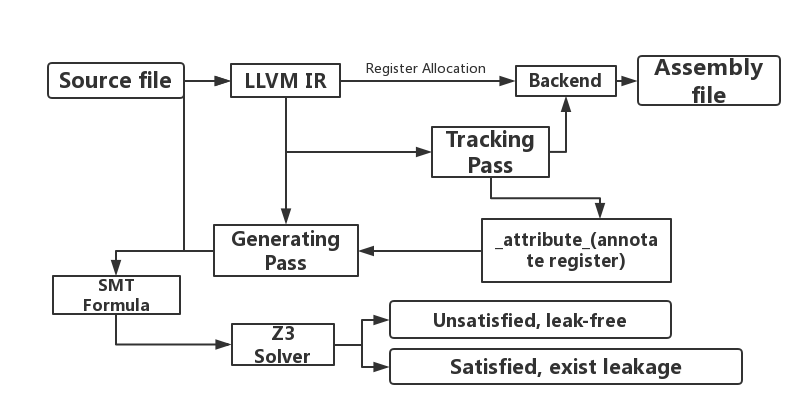
\includegraphics[totalheight=5.3cm]{detection.png}}
\caption{Overview of Detection Process (Zoom in for detail)}
\label{detection}
\end{figure}
Firstly, the Tracking pass will monitor the register allocation process in the backend, and gather such information. For instance, if intermediate variables \emph{v1} and \emph{v2} are not showing up in the same live-variable set of each instruction, then \emph{v1} and \emph{v2} can be distributed into same register. Tracking pass will annotate such variables sharing the same register, and transmit this annotated information to another Generating pass. Generating pass will accept the input from \emph{IR} file and the annotated information from the Tracking pass, and return the SMT formula. The SMT formula for verifying whether the power consumption of program differs with respect to \emph{key} are illustrated as below.\\
$${ \varphi  }_{ diff }=\exists { k }_{ 1 },{ k }_{ 2 }, { k }_{ 1 }\neq { k }_{ 2 }\wedge ( \sum _{ x\in P }{ I({ x },{ k }_{ 1 }) } \neq \sum _{ x\in P }{ I(x,{ k }_{ 2 }) } \vee {\varphi}_{RegReuse} ) $$ \\
${ \varphi  }_{ diff }$ represents whether the formula that the power consumption of program will differ according to the different \emph{key}. Given various \emph{key}, it's necessary to check both the sum of all possible intermediate values and the sum of transitions of all the registers are different. $\sum _{ x\in P }{ I(x,{ k }_{1}) } $ represents the sum of all variable values under possible permutations of the input $x$ and ${k}_{1}$. While ${\varphi}_{RegReuse}$ means that if the variables have reused the same register, then if the value transitions of the same register depend on \emph{key}, which can also imply that the source program exists \emph{key}-induced difference of power consumption. $f(I)$ equals to true if intermediate variable \emph{I} shares the same register with other variables, vice versa.
$${\varphi}_{RegReuse} = (f(I)\wedge \sum _{ x\in P }{ \Delta I(x,{ k }_{ 1 })\neq \sum _{ x\in P }{ \Delta I(x,{ k }_{ 2 }) }  } ) $$

% something to comment
\begin{comment}
\If {$i > \textit{stringlen}$} \Return false
\EndIf
\State $j \gets \textit{patlen}$
\end{comment}

\algdef{SE}[DOWHILE]{Do}{doWhile}{\algorithmicdo}[1]{\algorithmicwhile\ #1}%

\begin{algorithm}
\caption{Leakage Detection}\label{euclid}
\begin{algorithmic}[1]
\Procedure{Detection}{}
\State $\textit{M} \gets \text{number of }\textit{intermediate variables}$
\State $\textit{N} \gets \text{number of }\textit{possible permutations I}$
\State $i \gets \textit{iterator of instructions inside the function}$
\State $\textit{Sum, ${Transition}_{sum}$} \gets \textit{Output}$
\BState \emph{Initialize}:
\State $ \textit{Reg} \gets \textit{${Map}_{VR}(var)$} $ 
\State $ \textit{Var} \gets \textit{${Map}_{RV}(reg)$}$
\BState \emph{loop}:
\If {$\textit{inst\_iterator i } \neq \textit{inst\_end()}$}
	\If {$\textit{I }$ is annotated}
	\State $\textit{f(I)} \gets \textit{True}$ 
	\EndIf
\State \textbf{goto} \emph{loop}.
\State \textbf{close};
\EndIf
\State $\textit{cnt\_n} = 0, \textit{cnt\_m} = 0$
\Do
  \State $cnt_m += 1$
   \Do
    \State $cnt_n += 1$
    \State $Ivar = {Intermediate}_{var}(cnt\_n)$
    \State $Sum(cnt\_m) += Ivar$
    	\State $VarNext = {Map}_{RV}(++{Map}_{VR}(Ivar))$
	\State $delta = f(I)?VarNext:0$
	\State ${Transition}_{Sum}(cnt\_m) += delta$
    \doWhile{$cnt\_n \neq N$}
  \doWhile{$cnt\_m \neq M$} 
 \EndProcedure
\end{algorithmic}
\end{algorithm}

\subsection{New Countermeasure}
%We explain how our new method works and why it can eliminate the new leakage... 
The initial state and state transition in the same register is related to power consumption. The new-found leakage arises from the fact that different \emph{key} values can induce different state transitions, thus power consumption also changes. As we can see from Figure~\ref{example2}, in line 11, \%edx initially stores the \emph{key} value. Under HW model, the number of 1-bit in register will influence the power consumption, hence, different \emph{key} values will induce the difference in power consumption of register \%edx. In Line 10-11, state transition of the register \%edi is dependent on \emph{key}. Under HD model, the number of 1-0 transitions in register correlates to the power consumption, therefore, \emph{key}-induced state transition in register \%edi is also related to the power consumption.
\\
For solving those leakages in power channel, we must ensure that the \emph{key} is independent of the power consumption. Based on the HW and HD model, we've proposed a mitigation method which spills the \emph{key} value and intermediate result directly related to \emph{key} into memory. There are two reasons for this solution: Firstly, in X86 instructions, the operands of the operation can be a register or memory location. If we put the \emph{key} in one register, it's obvious the power consumption of this register is dependent on \emph{key}. Hence, we store \emph{key} in memory before calculation. Secondly, in Section D, we propose that due to the fact that multiple intermediate variables are allocated in the same register, hence the state transition is related to \emph{key}. If we allocate distinct registers to intermediate variables, the problems still exist. Because most arithmetic instructions are 2-operand design, which means that it's possible one register representing both the source operand and the result operand. Hence, for one instruction, the state transition from the source value to result value is related to another value stored in other locations. As the \emph{key} has been stored in memory, if we put the \emph{key}-related calculation result into another register such as \emph{R}, then the transition of \emph{R} is dependent on \emph{key}, which still owns the power channel leak. Hence, we also put the \emph{key}-related result into memory. (The solution is based on the assumption that the value or value transitions of the register correlate with the power consumption while the memory does not.) \\
\begin{figure}[hbt!]
\centering
\begin{minipage}{.65\linewidth}
\begin{lstlisting}[language={[ANSI]C},numbers=left,numberstyle=\tiny, basicstyle=\ttfamily\small, frame=none]
leak:                                   # @leak
	.cfi_startproc
# BB#0:                                 # %entry
	pushq	%rbx
.Ltmp2:
	.cfi_def_cfa_offset 16
.Ltmp3:
	.cfi_offset %rbx, -16
	movl	%edi, %ebx
	xorl	%esi, %ebx
	xorl	$1, %ebx
	xorl	%ebx, 24(%esp)
	movl	%ecx, %ebx
	andl	24(%esp), %ebx
	movl	$.L.str, %edi
	xorl	%eax, %eax
	movl	%ebx, %esi
	callq	printf
	movl	%ebx, %eax
	popq	%rbx
	ret
\end{lstlisting}
\end{minipage}
\caption{Mitigation of Example1 assembly code on X86-64}
\label{example3}
\end{figure}
Hence, after modifying the register allocation, the secure assembly code is as Figure~\ref{example3}. In Figure~\ref{example3}, we put \emph{key} value in the stack(24(\%esp)), and stores the \emph{key}-directly-related result in the same memory position as \emph{key} is out of the live range after line 16. Later, to avoid the state transition of register \%ebx has some relation with \emph{key}, we put another input variable \emph{i3} in this register \%ebx instead of the \emph{key}-directly-related result. After that we execute Line 6 in Figure~\ref{example1}, load the intermediate variable \emph{n2} stored in memory, and execute the \emph{and} operation with the \emph{i3} stored in register \%ebx. Finally, the output result is in \%ebx. In this way, both the initial state and the state transition of the register has no correlation with \emph{key}.
%\section{Implementation \&\& Experiment Result}

\section{Conclusion}
As previous methods didn't consider the register allocation scenarios under the Hamming Distance power analysis model, therefore they fail to mask the potential power-channel leakage program. This paper propose a more precise leakage model for verifying whether the given program exist power channel leakage after the register allocation phase. Meanwhile, we also propose a mitigation approach for generating the leak-free program by designing a secure register allocation phase, which put the public data into the register as usual and spill the sensitive data into memory to protect the attacker from inferring the \emph{key} by some techniques such as differential power analysis.
\begin{table}[]
\resizebox{\columnwidth}{!}{
\begin{tabular}{|l|l|l|l|l|l|l|l|}
\hline
Benchmark & Name                                          & Detection Time & HD\_SENSITIVE & EC Time(before) & EC Time(after) & MEM (before) & MEM (after) \\ \hline
P3        & CHES13 AES Shift Rows                         & 0.267s         & NO            &                 &                &              &             \\ \hline
P4        & CHES13 Messerges Boolean to Arithmetic (bit0) & 0.353s         & NO            &                 &                &              &             \\ \hline
P5        & CHES13 Goubin Boolean to Arithmetic (bit0)    & 0.401s         & YES           & 0.003s          & 0.005s         &              &             \\ \hline
P6        & Masked AES Byte Version                       & 1.375s         & YES           & 0.007s          & 0.004s         &              &             \\ \hline
\end{tabular}
}
\end{table}

\bibliographystyle{plain}
\bibliography{refer.bib}

\end{document}
